\documentclass[11pt]{exam}
\usepackage[spanish]{babel}
\usepackage[utf8]{inputenx}
\usepackage{fontenc}
\usepackage{textcomp}
\usepackage{lmodern,pifont}
\usepackage{graphicx}
\graphicspath{ {./img_1479/} }
\usepackage{setspace}
\usepackage[dvipsnames]{color}
\usepackage{colortbl}
\usepackage{caption}
\usepackage{amsmath}

\newcommand\titexam[1]{\centering%
\fbox{\parbox{\textwidth}{\huge \sffamily \textbf{#1}}}\normalsize \vspace{1em}}

\renewcommand{\solutiontitle}{\noindent\textbf{Solución:}\par\noindent}

\pagestyle{empty}
\begin{document}
{\fontfamily{lmss}\selectfont
\textbf{INSTRUCCIONES:}
\begin{itemize}
    \item Se dispone de dos horas para responder las 20 preguntas.
    \item Cada pregunta tiene un valor de 0.5 punto.
    \item Para considerar la respuesta como correcta, la opción escogida ha de
      estar correctamente señalada. Las preguntas erróneamente marcadas se
      considerarán como incorrectas. 
    \item Cada respuesta incorrecta resta 0.17 puntos. Las respuestas en blanco no restan. 
\end{itemize}
\vspace{1cm}

\titexam{MF1479\_2 Propagación de plantas en vivero}
\begin{questions}
  % 1
\question El nombre científico de una especie se forma de dos partes. ¿Puedes
indicar a que categoría taxonómica corresponde la primera parte?
\begin{checkboxes}
  \choice A. Al Reino
  \choice B. A la Familia
  \CorrectChoice C. Al Género
  \choice D. Ninguna es correcta
\end{checkboxes}
% 2
\question ¿Qué tipo de raíz aparece en la imagen?
  \begin{figure}[h!]
    \centering
    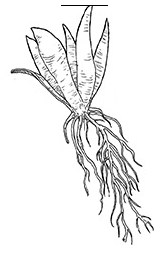
\includegraphics[width=0.2\textwidth]{fasciculada.PNG}
  \end{figure}
  \begin{checkboxes}
    \choice A. Napiforme
    \choice B. Pivotante
    \choice C. Ramificada
    \CorrectChoice D. Fasciculada
  \end{checkboxes}
\end{questions}
}
\end{document}
%%% Local Variables:
%%% mode: latex
%%% TeX-master: t
%%% End:
